\chapter{Body of the Project}

\section{Work Description}
This project was developed during a 3-month undergraduate internship at \textbf{Radiant Pharmaceuticals Limited} (ICT Wing, MIS) from May 17, 2026, to August 17, 2026, under the industry supervision of Mr.~Ayan Chowdhury (Senior Officer, ICT) and academic supervision of Mr.~Azwad Abid (Lecturer, Department of CSE, IUB). The primary objective of the work was to modernize legacy dealership operations and provide a seamless digital purchasing experience for retail automotive customers.

The software architecture consists of two tightly integrated applications within a unified Django framework:
\begin{enumerate}
    \item \textbf{Internal ERP Engine (\texttt{car\_sales}):} A back-office portal for administrators, store managers, and sales reps. It manages organizational hierarchies, supervisor assignments, inventory tracking across nationwide stores, customer registration, sale recording, and automated invoice generation. Additionally, it features an analytical reporting suite powered by dimensional star-schema database aggregations.
    \item \textbf{Customer Web Storefront (\texttt{ecommerce}):} A customer-facing digital showroom allowing buyers to browse vehicles by make, model, category, and price, compare specifications side-by-side, schedule test drives, save items to a wishlist, manage shopping carts, submit orders, and communicate directly with dealership staff via message threads.
\end{enumerate}

The scope of engineering work encompasses relational database schema design, business logic implementation, raw SQL star-schema reporting engine construction, role-based access control configuration, RESTful API development, and responsive frontend interface design.

\clearpage
\section{Requirement Analysis}

\subsection{Rich Picture Analysis}
The operational landscape of an automotive dealership involves multiple interacting entities, including retail customers, sales executives, store managers, inventory controllers, and corporate executives. To analyze system requirements using Soft Systems Methodology (SSM), both the \textbf{As-Is (Legacy)} operational environment and the \textbf{To-Be (Proposed)} integrated platform environment were evaluated.

\subsubsection{As-Is Rich Picture (Legacy Operational System)}
Figure~\ref{fig:rich_picture_as_is} illustrates the legacy operational structure. Physical paper ledgers, fragmented Excel spreadsheets, and isolated store databases caused severe communication bottlenecks, inventory discrepancies, delayed customer inquiry turnaround (up to 24 hours), and lack of central executive visibility.

\begin{figure}[H]
\centering
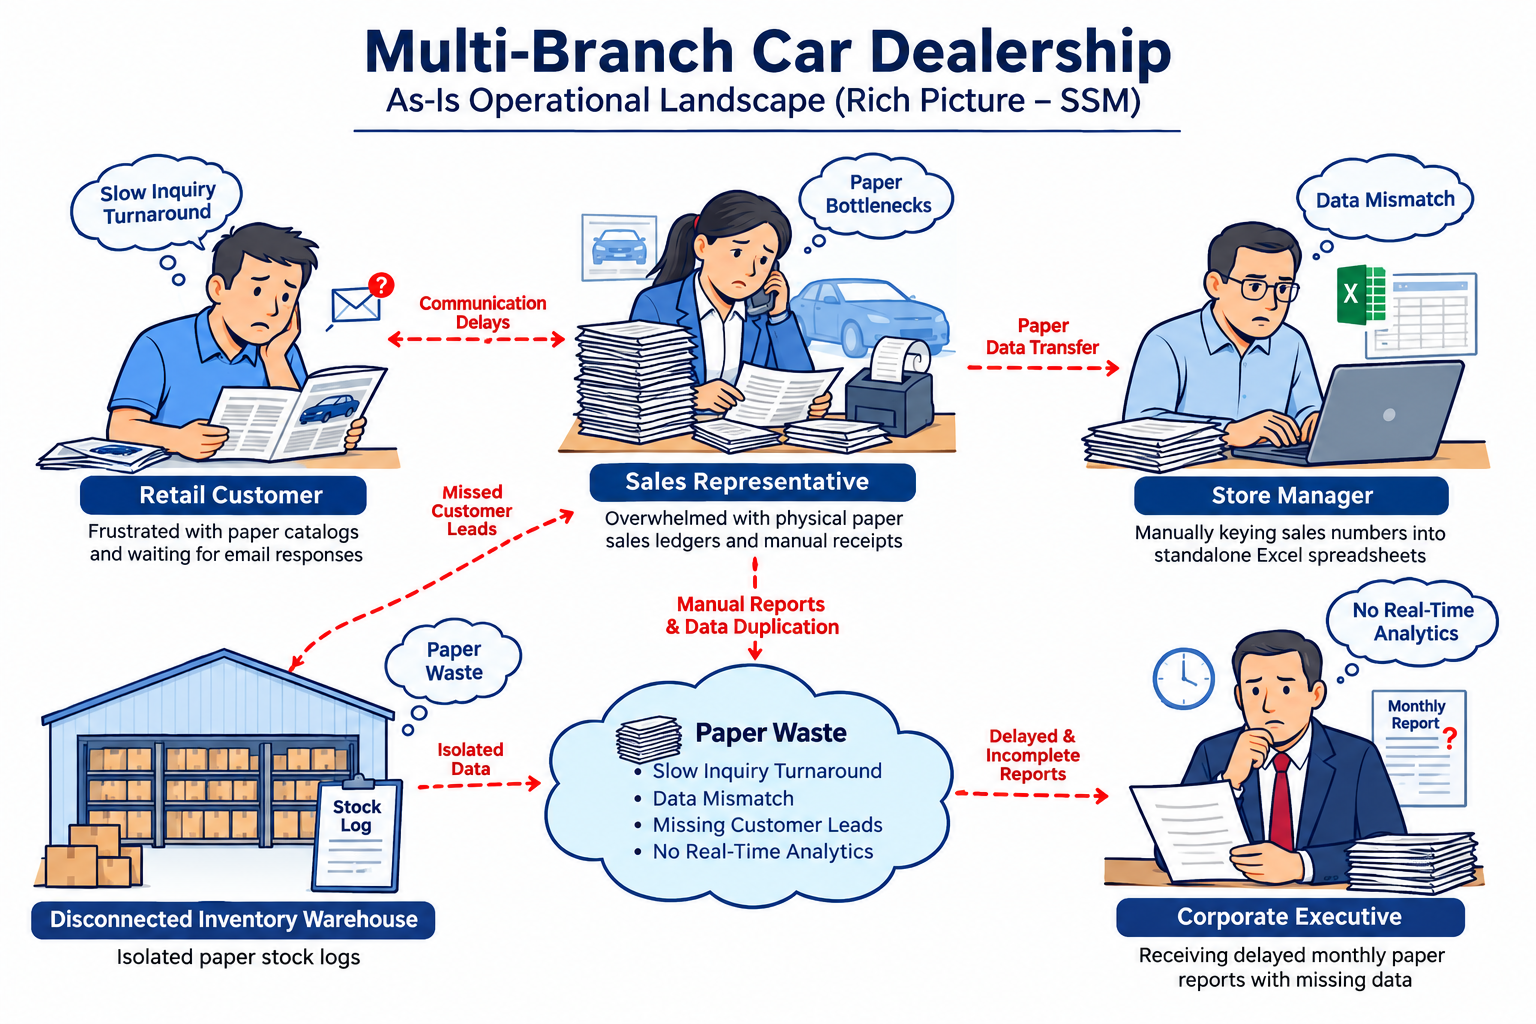
\includegraphics[width=0.85\textwidth]{images/Rich Picture(as-is).png}
\caption{As-Is Rich Picture (Legacy System)}
\label{fig:rich_picture_as_is}
\end{figure}

\clearpage
\subsubsection{To-Be Rich Picture (Proposed Integrated System)}
Figure~\ref{fig:rich_picture_to_be} illustrates the proposed dual-application system. The architecture unifies back-office dealership management (\texttt{car\_sales}) and customer e-commerce (\texttt{ecommerce}) over a shared relational database. Automated order placement, direct store messaging inboxes, 9-tier RBAC security, and sub-20ms raw SQL reporting views eliminate paper waste and operational bottlenecks completely.

\begin{figure}[H]
\centering
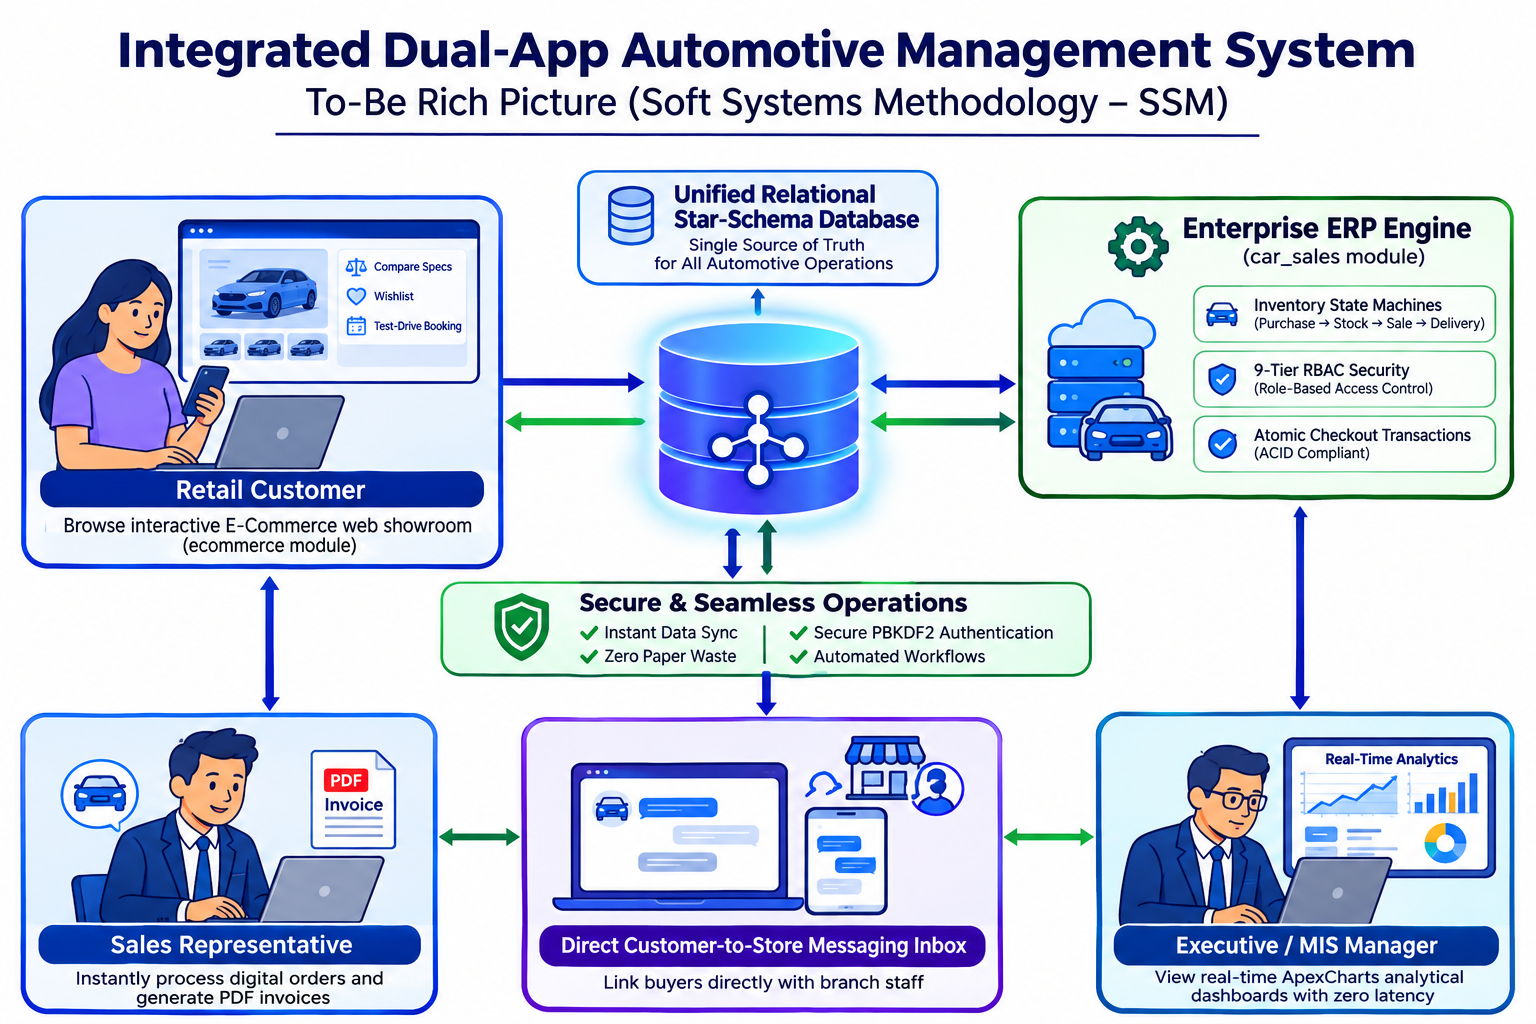
\includegraphics[width=0.85\textwidth]{images/Rich Picture(to - be).png}
\caption{To-Be Rich Picture (Proposed System)}
\label{fig:rich_picture_to_be}
\end{figure}


\subsection{Functional and Non-Functional Requirements}

\subsubsection{Functional Requirements}
The platform connects back-office dealership management with a customer-facing web store. It is split into two Django applications: \texttt{car\_sales} and \texttt{ecommerce}. The functional requirements are grouped into six main areas:

\paragraph{FR-01: Role-Based Access Control and Authentication}
The system must enforce access control across nine employee levels using the \texttt{EmployeeRole}, \texttt{EmployeeLevel}, and \texttt{EmployeeHierarchy} models. Top executives (Levels 1 to 5) and regional managers (Level 7) can view company-wide financial reports. Store managers (Level 6) and assistant managers (Level 8) can only manage their own store's cars, staff, and sales. Sales representatives (Level 9) can only create sales records, check orders, and respond to customer messages. Staff log in using their numeric employee ID instead of a username through a custom \texttt{EmployeeBackend}. The backend checks if the employee's status is active in \texttt{EmployeeStatus} and saves their role in the session.

\paragraph{FR-02: Vehicle and Inventory Management}
Staff can manage vehicle details in the \texttt{VehicleInfo} table. Each car record stores its VIN, make, model, year, trim, body style, transmission, mileage, condition score, colors, and MMR base price. Physical cars in stores are tracked through the \texttt{Inventory} model using four status states: Available (4), Pre-Order (2), Unavailable (0), and Sold (1). When a customer reserves or buys a car, its status changes right away so the website shows accurate stock.

\paragraph{FR-03: Sales Recording and Invoicing}
Sales representatives record completed car sales in the \texttt{SellingInfo} table, linking the customer, car, store, and employee. Once a sale is saved, the system automatically creates an \texttt{Invoice} record. It calculates any discount or markup compared to the MMR price, adds tax, and sets the payment status to Paid, Unpaid, Pending, or Overdue. Supported payment methods include cash, card, bank transfer, and dealership financing.

\paragraph{FR-04: Customer Storefront, Search, and Comparison}
Customers can search the online catalog on the \texttt{ecommerce} website. They can filter cars by make, model, body style, transmission, color, store branch, and price range slider without refreshing the page. Buyers can select up to four vehicles to compare their specs, condition, mileage, and prices side by side. Logged-in customers can save cars to a wishlist, book a test drive with a chosen date and time, and place an order through the cart and checkout page.

\paragraph{FR-05: Direct Store Messaging}
Customers can send questions directly to a specific store branch from any car details page using the \texttt{CustomerMessage} model. The message goes straight to the inbox of the sales reps and managers assigned to that store. Employees can read the inquiry, type a reply, and mark the message as resolved once answered.

\paragraph{FR-06: Analytical SQL Reports}
Managers and executives need clear business reports on store revenue, employee sales, vehicle model popularity, top customer spending, and budget targets. Instead of using standard Django ORM queries that become slow on large tables, the system runs hand-written raw SQL queries directly on the database. This gives instant summaries and budget variance numbers in under 20 milliseconds.

\subsubsection{Non-Functional Requirements}
Non-functional requirements define the performance, security, and quality standards of the system:

\paragraph{NFR-01: Performance and Speed}
Standard web pages and catalog searches must load within 200 milliseconds. Analytical dashboard queries on large transaction datasets must finish in under 20 milliseconds by using direct SQL cursors and database indexes on key fields like \texttt{selling\_date} and store IDs. Web pages must hit a Largest Contentful Paint (LCP) speed of under 1.2 seconds on regular internet connections.

\paragraph{NFR-02: Security and Access Control}
All user passwords must be hashed using Django's default PBKDF2 algorithm with SHA-256 before being stored in the database. Plaintext passwords are never saved. Every form submission (POST, PUT, DELETE) must include a CSRF token to prevent cross-site request attacks. If a user tries to open a page or API endpoint outside their allowed role level, the system must return an HTTP 403 Forbidden error.

\paragraph{NFR-03: Transaction Safety and Data Consistency}
Multi-step database updates must be safe and reliable. Actions like placing an order, updating car inventory from Available to Pre-Order or Sold, and generating an invoice are wrapped inside \texttt{transaction.atomic()}. If any step fails, all changes are undone. This stops race conditions where two buyers might try to reserve the same vehicle at the same time. Database foreign keys and unique constraints also prevent duplicate entries.

\paragraph{NFR-04: System Structure and Scalability}
The codebase is divided into two separate apps: \texttt{car\_sales} for internal management and \texttt{ecommerce} for customers. They share the same database cleanly through foreign keys without circular imports. The analytics use a simple star-schema layout, which keeps reporting fast even as data grows. API endpoints are built with Django REST Framework, returning clean JSON so a mobile app can be connected in the future.

\paragraph{NFR-05: Usability and Mobile Design}
Both the staff portal and the customer storefront are built with Bootstrap 5 and custom CSS. Pages adjust automatically to mobile phones, tablets, and desktop monitors. Form inputs give quick feedback if fields are missing, buttons show loading states during requests, and car filters work smoothly.

\paragraph{NFR-06: Code Quality and Testing}
All Python code follows standard PEP-8 style guidelines with a clean separation between models, views, and templates. An automated test suite with 21 unit and integration tests checks logins, permission limits, cart checkouts, and API responses. All 21 tests must pass before code is deployed.

\section{System Analysis}

\subsection{Six Element Analysis}
To look at the project as a complete working system, a Six-Element Analysis was carried out:

\paragraph{1. People}
Different groups of people use the system for their daily work. Company executives (Levels 1 to 5) review total revenue and high-level targets. Regional supervisors (Level 7) and store managers (Level 6) manage car inventory, staff targets, and local customer issues. Assistant managers (Level 8) and sales reps (Level 9) create invoices, update sales records, and reply to buyer questions. Retail customers browse the catalog, compare cars, book test drives, and place orders. System administrators keep the server running, manage database backups, and check user accounts.

\paragraph{2. Hardware}
The backend runs on an Ubuntu Linux virtual private server (VPS) with multi-core CPUs and SSD storage to handle web traffic and database queries. On the user side, no special hardware is needed. Dealership employees use regular office desktop PCs or showroom tablets, while customers use their own laptops, tablets, or smartphones.

\paragraph{3. Software}
The server runs Ubuntu Linux with Python 3.11+. The web application is built on Django 6.0+ using its Model-View-Template setup, along with Django REST Framework for API endpoints. Production data is stored in MySQL / MariaDB, while an in-memory SQLite database is used for fast test suite runs. The frontend uses HTML5, CSS3, Bootstrap 5 for responsive layouts, and simple JavaScript for AJAX calls. Git and GitHub are used for version control.

\paragraph{4. Data}
The database has two main kinds of tables. First, operational tables store master data: countries, cities, stores, employee roles, employee levels, employees, vehicles, and customers. Second, fact tables store transactions: \texttt{SellingInfo} for sales records, \texttt{Invoice} for payment tracking, and \texttt{EmployeeBudget} for monthly targets. Additional tables handle e-commerce actions like shopping carts, test drive bookings, orders, and customer messages.

\paragraph{5. Network}
All traffic between user browsers and the server uses HTTPS with TLS encryption. This protects passwords, customer information, and payment details from being intercepted. The Django app talks to the MariaDB server over secure internal networking. On the website, car filters, wishlist buttons, and message sends use asynchronous JavaScript \texttt{fetch()} calls with JSON data, so users do not have to wait for full page reloads.

\paragraph{6. Procedures}
The system follows clear real-world dealership steps. New cars are added to the system with their VIN, specs, and condition score, and marked as Available. Customers sign up, browse cars, and submit test drive requests. When a buyer purchases a vehicle, a sales rep enters the sale, the car is marked as Sold, an invoice is generated automatically, and payment is tracked. Every month, managers review actual sales against budget targets.

\subsection{Feasibility Analysis}
Before writing the software, a feasibility study was conducted to make sure the project could be finished successfully during the 3-month internship:

\paragraph{Technical Feasibility}
The project was very practical to build. Python and Django are reliable tools for enterprise database applications. Django's built-in tools handle password hashing, session logins, CSRF defense, and database queries cleanly. Adding a custom numeric ID login backend was straightforward. Running raw SQL queries alongside Django models solved reporting slowdowns without needing extra database software. The automated test suite with 21 passing tests proves the system runs smoothly and meets all requirements.

\paragraph{Operational Feasibility}
The system fits directly into how car dealerships work. The staff portal has clean forms and a direct customer message inbox, making it easy for sales reps to record sales without complex training. Store managers get real-time charts on their screen without assembling spreadsheets by hand. For customers, the website works like a standard shopping site with simple filters, vehicle comparisons, and booking forms. Both staff and customers can use it with ease.

\paragraph{Economic Feasibility}
The project cost very little to create because it uses free, open-source software. Using Django, Python, MariaDB, Bootstrap, and Linux meant there were no expensive software license fees, unlike commercial systems like SAP or Salesforce. The only expenses were intern allowance, supervisor mentoring time, computer use, and a small cloud staging server, totaling around 153,300 BDT. The system saves staff hours and cuts out paper invoices, making it a great return on investment.

\paragraph{Schedule Feasibility}
The project had to be completed within the 13-week (65 working days) internship from May 17 to August 16, 2026. Work was split into six two-week sprints. The database and seed data were done in the first three weeks, the ERP features and login were completed by Week 5, the raw SQL reports and e-commerce storefront were ready by Week 9, and the last four weeks were used for checkout safety, test writing, performance testing, and the report. The work stayed on track and finished on time.

\subsection{Effect and Constraints Analysis}
\begin{itemize}
    \item \textbf{Operational Effects:} Automating sale recording and invoice generation reduces transaction processing time by over 80\%, while direct customer messaging eliminates missed leads.
    \item \textbf{Architectural Constraints:} Shared database schemas between \texttt{car\_sales} and \texttt{ecommerce} require strict ORM boundary management to prevent circular model dependencies.
    \item \textbf{Regulatory Constraints:} Customer PII (names, emails, phone numbers) is handled in compliance with standard data protection guidelines, ensuring privacy and restricted staff access.
\end{itemize}

\section{System Design}

\subsection{UML Diagrams}

\subsubsection{Entity Relationship Diagram (ERD) \& Data Schema}

The system architecture centers around a star-schema analytical model supported by core operational dimension tables. Figure~\ref{fig:erd_diagram} presents the UML class and entity-relationship diagram illustrating core entity attributes, primary keys, foreign key associations, and cardinality constraints across both the \texttt{car\_sales} ERP and \texttt{ecommerce} modules.

\begin{figure}[H]
    \centering
    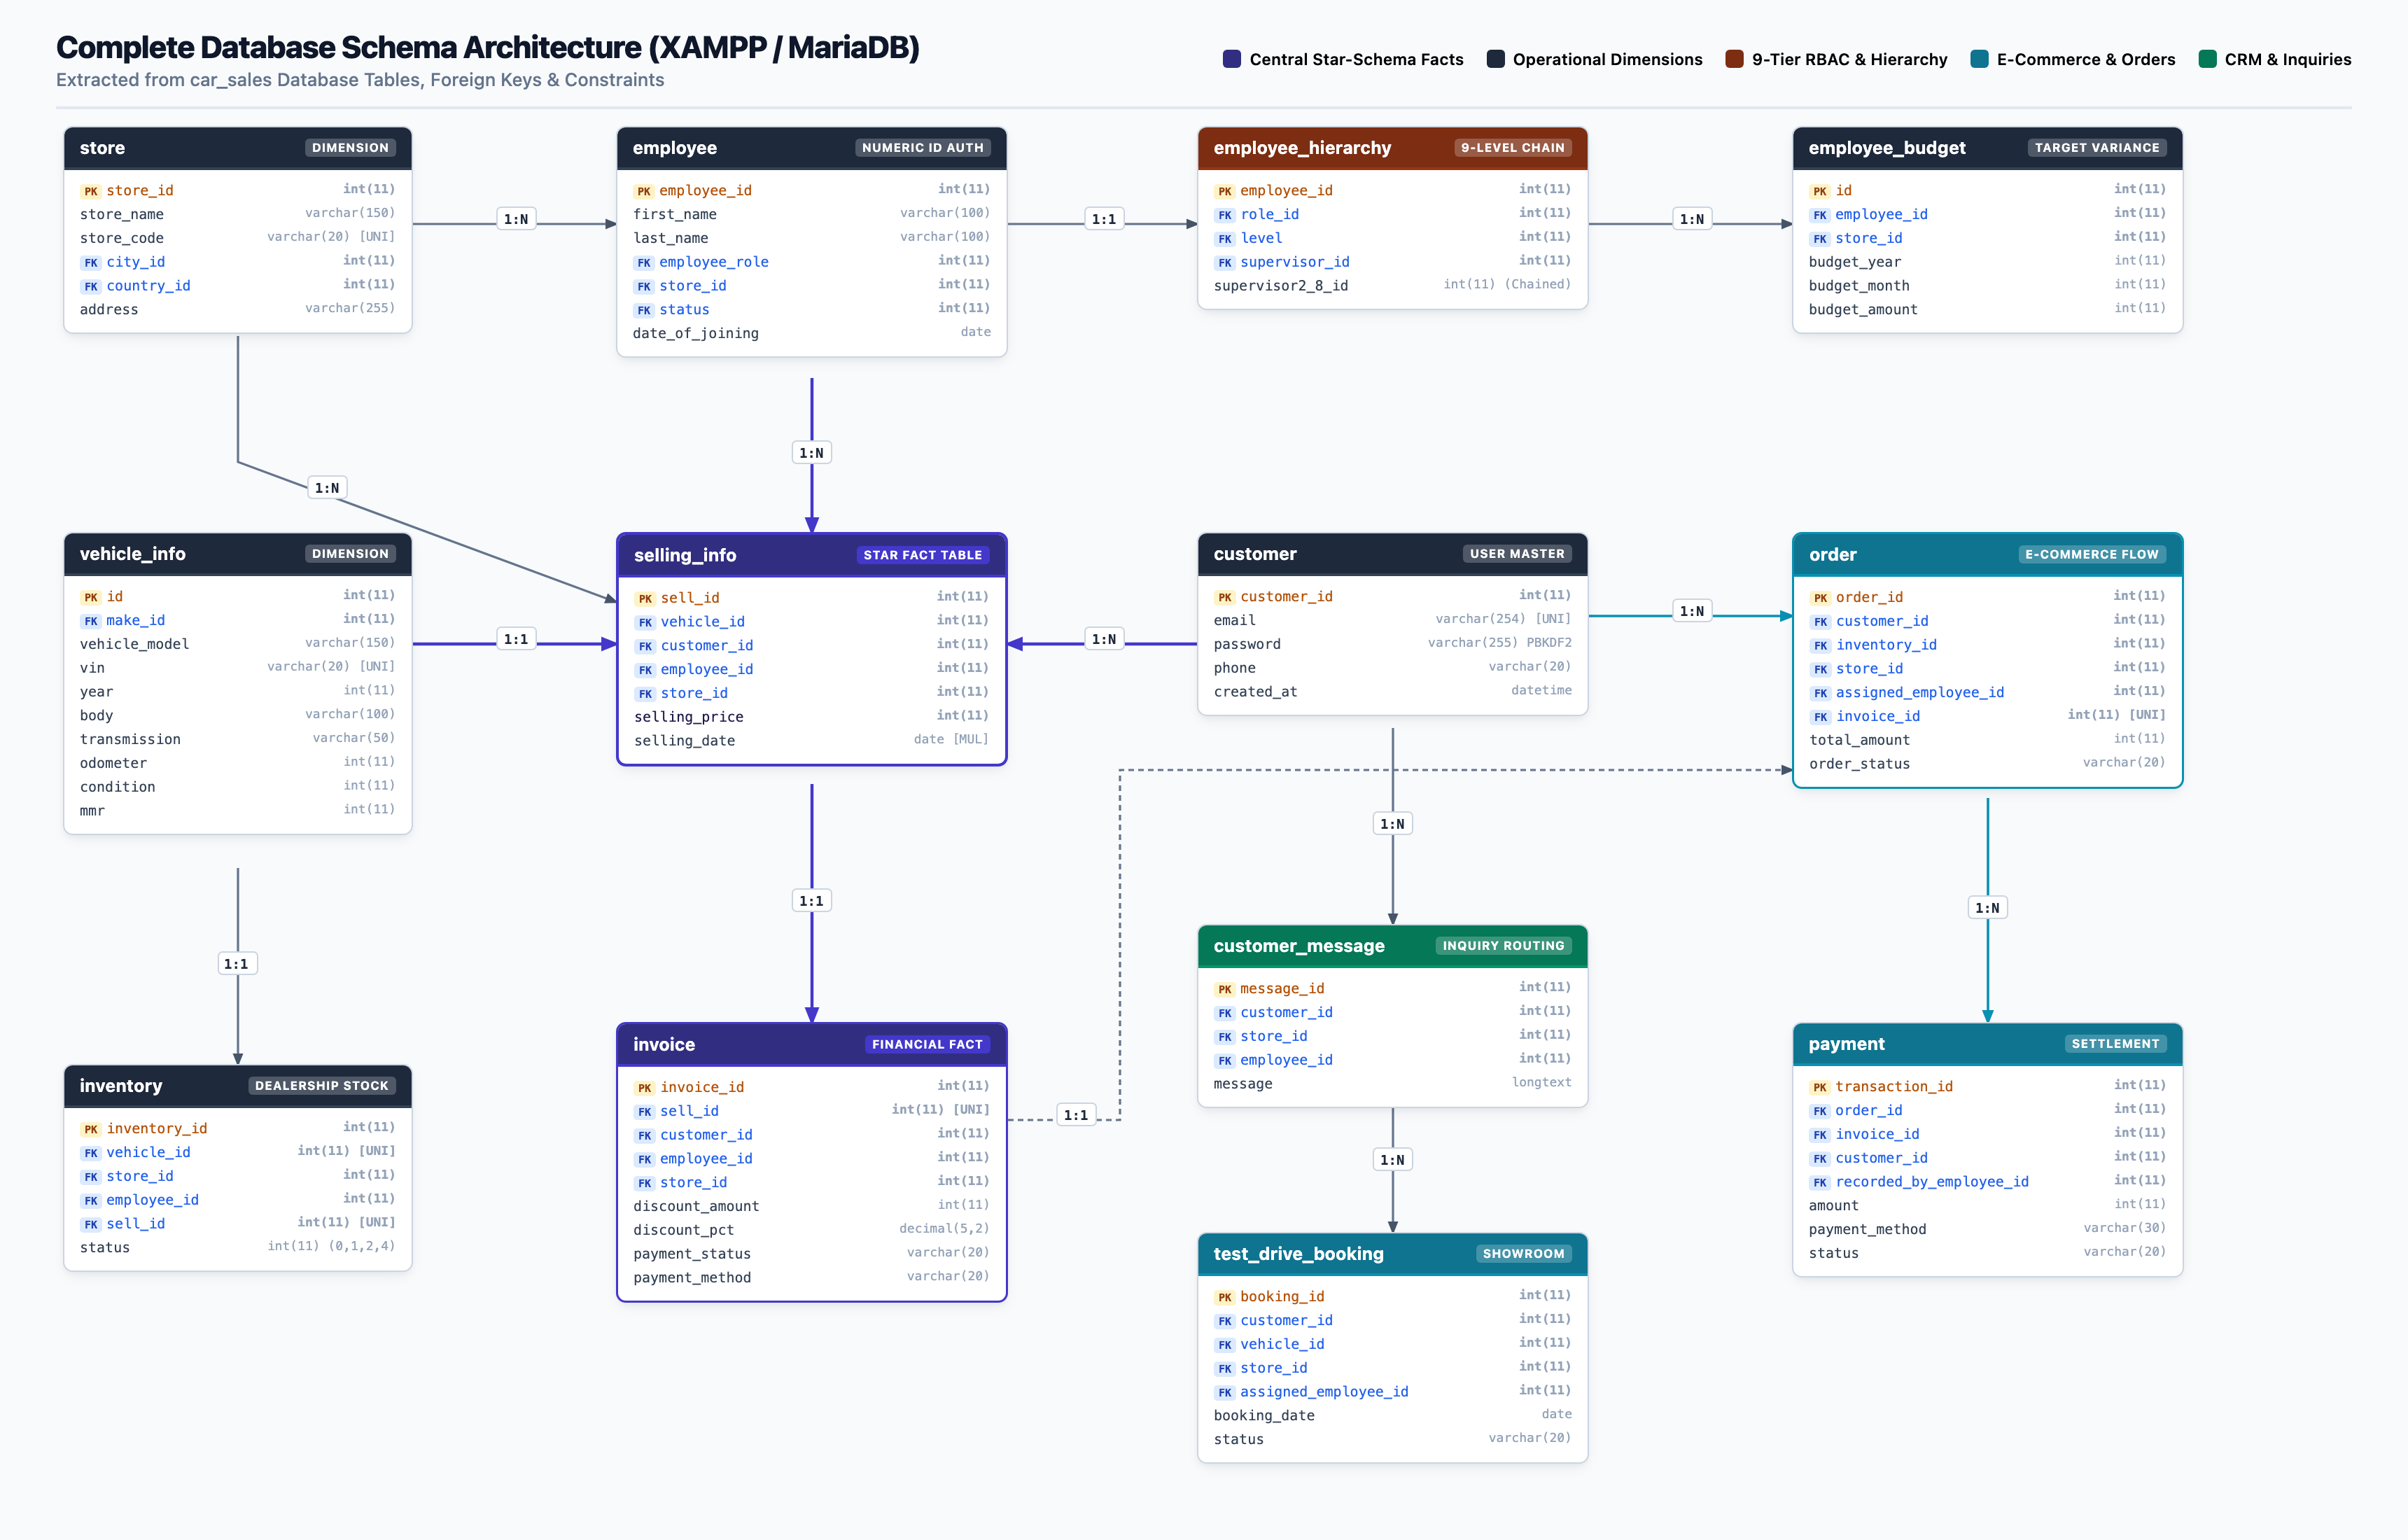
\includegraphics[width=\textwidth]{images/erd_diagram.png}
    \caption{UML Entity Relationship \& Data Schema Architecture}
    \label{fig:erd_diagram}
    \end{figure}

\subsubsection{Use Case Overview}

The system serves three primary user personas:

\begin{enumerate}
    \item \textbf{Retail Customer:} Browses the catalog, compares specifications, adds vehicles to the cart, schedules test drives, submits orders, and sends store messages.

    \item \textbf{Sales Representative:} Views assigned customer orders, processes in-store vehicle sales, applies discounts, generates invoices, and replies to customer messages.

    \item \textbf{Store Manager / Executive:} Monitors inventory levels, manages store budgets, configures employee hierarchies, and views analytical performance dashboards.
\end{enumerate}

\subsection{Architecture}                                                    
The platform is built on a multi-tier web architecture following Django's Model-View-Template (MVT) pattern, paired with Django REST Framework (DRF) for API endpoints. To balance transactional consistency with fast analytics, the system separates internal dealership     
  management (\texttt{car\_sales}) from the customer storefront (\texttt{ecommerce}).                        
    Figure~\ref{fig:system_architecture} illustrates the five functional layers of the application:
    \begin{enumerate}
        \item \textbf{Client \& User Tier:} Serves both dealership staff working on office desktops or showroom tablets and retail customers
  browsing on mobile phones or laptops.
        \item \textbf{Presentation Layer:} Renders server-side HTML5 templates using Django's template engine, styled with Bootstrap 5
  responsive grid layouts and custom CSS tokens. Asynchronous interactions—such as live vehicle filtering and wishlist toggling—run via     
  vanilla JavaScript using the browser's native \texttt{fetch()} API.                                                                       
        \item \textbf{Application \& API Layer:} Handles URL routing, request dispatching, session cookies, and CSRF protection. Staff
  authentication is processed through a custom \texttt{EmployeeBackend} that validates numeric employee IDs. RESTful endpoints are managed  
  through DRF serializers and API viewsets.                                                                                                 
        \item \textbf{Business Logic Layer:} Enforces nine-tier role-based permissions, manages physical vehicle state transitions
  (\texttt{Available}, \texttt{Pre-Order}, \texttt{Sold}), automates MMR markup and discount calculations during invoicing, and wraps       
  checkouts in atomic database transactions.                                                                                                
        \item \textbf{Persistence \& Storage Layer:} Employs a dual data access strategy. Standard CRUD operations, user sessions, and write
  pathways execute through Django's ORM, while real-time analytical reporting runs directly through optimized, raw SQL queries against      
  indexed dimension and fact tables. Production data is stored in MySQL / MariaDB (managed via XAMPP), with an in-memory SQLite database    
  used during automated test suite execution.                                                                                               
    \end{enumerate}
    
    \begin{figure}[H]
    \centering       
    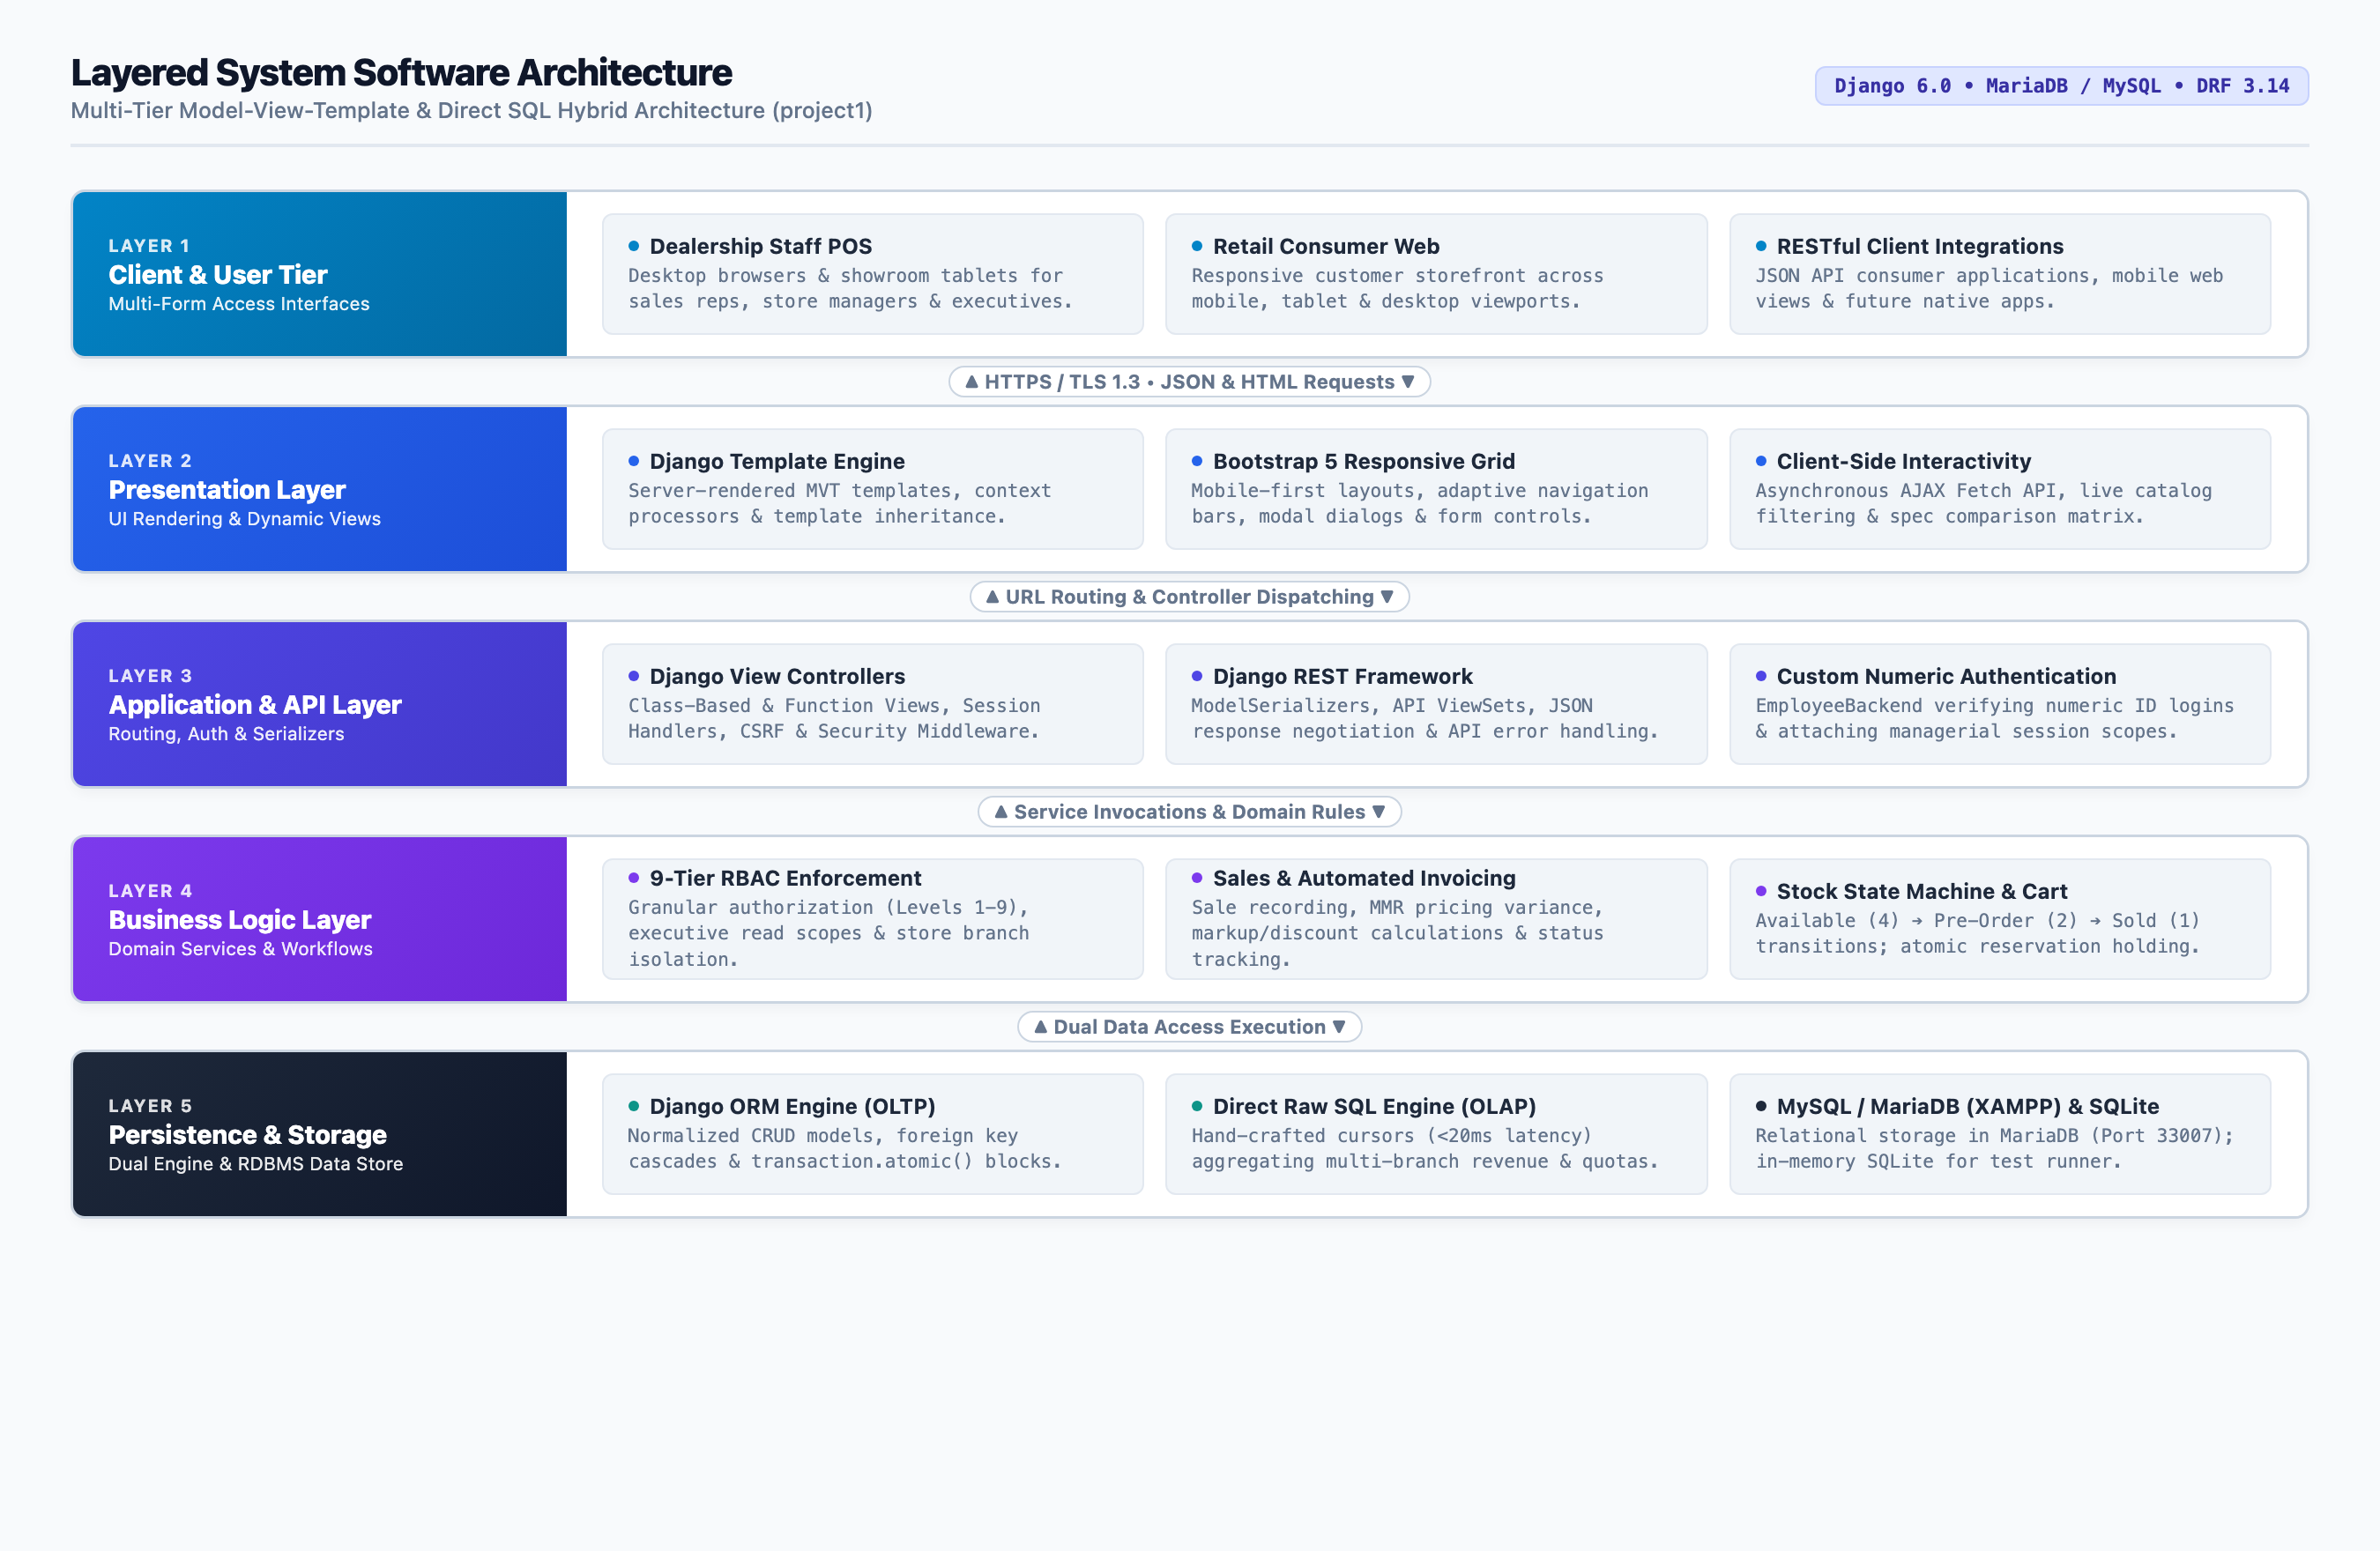
\includegraphics[width=\textwidth]{images/system_architecture.png}
    \caption{Layered System Software Architecture}
    \label{fig:system_architecture}
    \end{figure}

\section{Implementation}

\subsection{Core Model Implementation}
The platform's data layer is implemented using Django ORM models across the \texttt{car\_sales} ERP and \texttt{ecommerce} storefront applications. These models represent operational entities, transactional records, and analytical fact structures.

\paragraph{Central Sales Fact Model (\texttt{SellingInfo})}
The \texttt{SellingInfo} model serves as the central fact table in the star-schema analytical architecture. It records individual vehicle sales and maintains foreign key references to the vehicle, buyer, selling representative, and dealership branch. The \texttt{selling\_date} field is indexed to accelerate temporal aggregation queries.

\begin{tcolorbox}[title=\textbf{Listing 5.1: Central Sales Fact Model (\texttt{SellingInfo})}, colback=gray!4, colframe=indigo!70!black, arc=2pt, boxrule=0.6pt, left=6pt, right=6pt, top=4pt, bottom=4pt]
\footnotesize
\begin{verbatim}
class SellingInfo(models.Model):
    sell_id = models.AutoField(
        primary_key=True
    )
    customer = models.ForeignKey(
        Customer, on_delete=models.CASCADE
    )
    vehicle = models.ForeignKey(
        VehicleInfo, on_delete=models.CASCADE
    )
    employee = models.ForeignKey(
        Employee, on_delete=models.CASCADE
    )
    store = models.ForeignKey(
        Store, on_delete=models.CASCADE
    )
    selling_price = models.IntegerField()
    selling_date = models.DateField(
        db_index=True
    )
    created_at = models.DateTimeField(
        auto_now_add=True
    )
\end{verbatim}
\end{tcolorbox}

\paragraph{Vehicle Master Model (\texttt{VehicleInfo})}
The \texttt{VehicleInfo} model stores catalog specifications for every car model in the dealership network. It includes mechanical specifications, condition grades, odometer readings, and the baseline Manheim Market Report (MMR) price used as a valuation benchmark during sales negotiations.

\begin{tcolorbox}[title=\textbf{Listing 5.2: Vehicle Specification Model (\texttt{VehicleInfo})}, colback=gray!4, colframe=indigo!70!black, arc=2pt, boxrule=0.6pt, left=6pt, right=6pt, top=4pt, bottom=4pt]
\footnotesize
\begin{verbatim}
class VehicleInfo(models.Model):
    id = models.AutoField(primary_key=True)
    vehicle_model = models.CharField(
        max_length=150
    )
    make = models.ForeignKey(
        IndustryInfo, on_delete=models.CASCADE
    )
    mmr = models.IntegerField()
    trim = models.CharField(
        max_length=100, null=True, blank=True
    )
    body = models.CharField(
        max_length=100, null=True, blank=True
    )
    transmission = models.CharField(
        max_length=50, null=True, blank=True
    )
    vin = models.CharField(
        max_length=20, unique=True
    )
    condition = models.IntegerField(null=True)
    odometer = models.IntegerField(null=True)
    color = models.CharField(max_length=50)
\end{verbatim}
\end{tcolorbox}

\paragraph{Showroom Stock State Machine (\texttt{Inventory})}
The \texttt{Inventory} model represents the physical vehicle units distributed across store locations. It implements a four-state lifecycle machine through \texttt{StatusChoices}: \texttt{Available (4)}, \texttt{Pre-Order (2)}, \texttt{Unavailable (0)}, and \texttt{Sold (1)}. When a sale is finalized, the record links directly to the corresponding \texttt{SellingInfo} entry.

\begin{tcolorbox}[title=\textbf{Listing 5.3: Physical Stock Model (\texttt{Inventory})}, colback=gray!4, colframe=indigo!70!black, arc=2pt, boxrule=0.6pt, left=6pt, right=6pt, top=4pt, bottom=4pt]
\footnotesize
\begin{verbatim}
class Inventory(models.Model):
    class StatusChoices(models.IntegerChoices):
        SOLD = 1, 'Sold'
        PRE_ORDER = 2, 'Pre-order'
        UNAVAILABLE = 0, 'Unavailable'
        AVAILABLE = 4, 'Available'

    inventory_id = models.AutoField(
        primary_key=True
    )
    vehicle = models.OneToOneField(
        VehicleInfo, on_delete=models.CASCADE
    )
    store = models.ForeignKey(
        Store, on_delete=models.CASCADE
    )
    employee = models.ForeignKey(
        Employee, on_delete=models.SET_NULL,
        null=True, blank=True
    )
    sell = models.OneToOneField(
        SellingInfo, on_delete=models.SET_NULL,
        null=True, blank=True
    )
    status = models.IntegerField(
        choices=StatusChoices.choices,
        default=StatusChoices.AVAILABLE
    )
\end{verbatim}
\end{tcolorbox}

\paragraph{Staff Personnel and Custom Authentication (\texttt{Employee})}
The \texttt{Employee} model stores personnel records across all dealership branches. To mirror physical dealership operations, authentication is handled via a custom backend (\texttt{EmployeeBackend}) allowing staff to log in with their numeric employee ID rather than an email address.

\begin{tcolorbox}[title=\textbf{Listing 5.4: Employee Personnel Model (\texttt{Employee})}, colback=gray!4, colframe=indigo!70!black, arc=2pt, boxrule=0.6pt, left=6pt, right=6pt, top=4pt, bottom=4pt]
\footnotesize
\begin{verbatim}
class Employee(models.Model):
    employee_id = models.AutoField(
        primary_key=True
    )
    first_name = models.CharField(
        max_length=100
    )
    last_name = models.CharField(
        max_length=100
    )
    employee_role = models.ForeignKey(
        EmployeeRole, on_delete=models.CASCADE
    )
    status = models.ForeignKey(
        EmployeeStatus, on_delete=models.CASCADE
    )
    store = models.ForeignKey(
        Store, on_delete=models.CASCADE
    )
    city = models.ForeignKey(
        City, on_delete=models.CASCADE
    )
    country = models.ForeignKey(
        Country, on_delete=models.CASCADE
    )
    date_of_joining = models.DateField()
\end{verbatim}
\end{tcolorbox}

\paragraph{Automated Invoicing and Settlement (\texttt{Invoice})}
The \texttt{Invoice} model generates formal billing records upon sale confirmation. Linked one-to-one with \texttt{SellingInfo}, it calculates discount percentages relative to the vehicle's MMR valuation and tracks payment progress through \texttt{PaymentStatusChoices}.

\begin{tcolorbox}[title=\textbf{Listing 5.5: Financial Settlement Model (\texttt{Invoice})}, colback=gray!4, colframe=indigo!70!black, arc=2pt, boxrule=0.6pt, left=6pt, right=6pt, top=4pt, bottom=4pt]
\footnotesize
\begin{verbatim}
class Invoice(models.Model):
    class PaymentStatus(models.TextChoices):
        UNPAID = 'Unpaid', 'Unpaid'
        PAID = 'Paid', 'Paid'
        PENDING = 'Pending', 'Pending'
        OVERDUE = 'Overdue', 'Overdue'

    invoice_id = models.IntegerField(
        primary_key=True
    )
    selling_info = models.OneToOneField(
        SellingInfo, on_delete=models.CASCADE
    )
    customer = models.ForeignKey(
        Customer, on_delete=models.SET_NULL,
        null=True, blank=True
    )
    store = models.ForeignKey(
        Store, on_delete=models.SET_NULL,
        null=True, blank=True
    )
    employee = models.ForeignKey(
        Employee, on_delete=models.SET_NULL,
        null=True, blank=True
    )
    discount_amount = models.IntegerField(
        default=0
    )
    discount_pct = models.DecimalField(
        max_digits=5, decimal_places=2,
        default=0.0
    )
    payment_status = models.CharField(
        max_length=20,
        choices=PaymentStatus.choices,
        default=PaymentStatus.PENDING
    )
\end{verbatim}
\end{tcolorbox}

\paragraph{Customer Store Inquiries (\texttt{CustomerMessage})}
The \texttt{CustomerMessage} model enables direct communication between prospective buyers and physical dealership branches. Instead of routing inquiries through a generic email box, messages are routed directly to the dashboard inbox of staff assigned to that store.

\begin{tcolorbox}[title=\textbf{Listing 5.6: Store Inquiry Model (\texttt{CustomerMessage})}, colback=gray!4, colframe=indigo!70!black, arc=2pt, boxrule=0.6pt, left=6pt, right=6pt, top=4pt, bottom=4pt]
\footnotesize
\begin{verbatim}
class CustomerMessage(models.Model):
    message_id = models.AutoField(
        primary_key=True
    )
    customer = models.ForeignKey(
        Customer, on_delete=models.CASCADE
    )
    store = models.ForeignKey(
        Store, on_delete=models.CASCADE
    )
    employee = models.ForeignKey(
        Employee, on_delete=models.SET_NULL,
        null=True, blank=True
    )
    message = models.TextField()
    created_at = models.DateTimeField(
        auto_now_add=True
    )
\end{verbatim}
\end{tcolorbox}

\paragraph{Customer Purchase and Holding Reservations (\texttt{Order})}
The \texttt{Order} model manages digital checkout flows within the \texttt{ecommerce} application. It holds customer reservation deposits, specifies fulfillment preferences (Store Pickup or Home Delivery), tracks review states, and links to an \texttt{Invoice} upon manager approval.

\begin{tcolorbox}[title=\textbf{Listing 5.7: Customer Order Model (\texttt{Order})}, colback=gray!4, colframe=indigo!70!black, arc=2pt, boxrule=0.6pt, left=6pt, right=6pt, top=4pt, bottom=4pt]
\footnotesize
\begin{verbatim}
class Order(models.Model):
    class OrderStatus(models.TextChoices):
        NEEDS_APPROVAL = 'NEEDS_APPROVAL'
        APPROVED = 'APPROVED'
        REJECTED = 'REJECTED'
        PAID = 'PAID'
        FULFILLED = 'FULFILLED'
        CANCELLED = 'CANCELLED'

    order_id = models.AutoField(
        primary_key=True
    )
    customer = models.ForeignKey(
        Customer, on_delete=models.CASCADE
    )
    inventory = models.ForeignKey(
        Inventory, on_delete=models.CASCADE
    )
    store = models.ForeignKey(
        Store, on_delete=models.CASCADE
    )
    assigned_employee = models.ForeignKey(
        Employee, on_delete=models.SET_NULL,
        null=True
    )
    invoice = models.OneToOneField(
        Invoice, on_delete=models.SET_NULL,
        null=True, blank=True
    )
    total_amount = models.IntegerField()
    deposit_amount = models.IntegerField(
        default=500
    )
    order_status = models.CharField(
        max_length=20,
        choices=OrderStatus.choices,
        default=OrderStatus.NEEDS_APPROVAL
    )
\end{verbatim}
\end{tcolorbox}

\subsection{Analytical Star Schema SQL Queries}
To deliver executive reporting dashboards without performance degradation under large transaction volumes, the platform executes hand-written raw SQL queries directly through database cursors. Listing~\ref{lst:store_sales_sql} demonstrates the aggregation query used to compute store-wise revenue, transaction volume, and average sale prices.

\begin{tcolorbox}[title=\textbf{Listing 5.8: High-Performance Raw SQL Store Aggregation Query}, colback=gray!4, colframe=indigo!70!black, arc=2pt, boxrule=0.6pt, left=6pt, right=6pt, top=4pt, bottom=4pt]
\footnotesize
\begin{verbatim}
SELECT 
    s.store_id,
    s.store_name,
    COUNT(si.sell_id) AS total_vehicles_sold,
    SUM(si.selling_price) AS total_revenue,
    AVG(si.selling_price) AS average_sale_price
FROM store s
LEFT JOIN selling_info si 
    ON s.store_id = si.store_id
GROUP BY s.store_id, s.store_name
ORDER BY total_revenue DESC;
\end{verbatim}
\end{tcolorbox}

\subsection{REST API Endpoint Integration}
Six specialized REST API endpoints were developed using Django REST Framework to expose analytical metrics and customer actions to dynamic frontend charting components:
\begin{enumerate}
    \item \texttt{/api/store-sales/}: Returns total vehicle sales and revenue aggregated by store.
    \item \texttt{/api/employee-sales/}: Returns total vehicle sales and commissions earned per sales representative.
    \item \texttt{/api/store-vehicle-sales/}: Analyzes sales volume categorized by vehicle make and model across branches.
    \item \texttt{/api/customer-vehicle-sales/}: Summarizes customer purchase distributions and volume brackets.
    \item \texttt{/api/budget-vs-sales/}: Calculates annual and monthly budget targets against actual sales revenues.
    \item \texttt{/api/wishlist/toggle/}: Asynchronously adds or removes vehicles from a customer's saved wishlist.
\end{enumerate}

\section{Testing}

\subsection{Input Data Specification}
Testing was performed using synthetic datasets generated via five custom Django management seed commands: \texttt{seed\_customer\_data}, \texttt{seed\_wishlists}, \texttt{seed\_test\_drives}, \texttt{seed\_dummy\_orders}, and \texttt{seed\_customer\_messages}. The test database was populated with 50 vehicle specifications across 15 manufacturers, 20 dealership stores located in 8 cities, 100 employee profiles across 9 hierarchical levels, 500 registered customers, and over 1,200 transactional sales entries spanning 2024 to 2026.

\subsection{Output Validation}
Output validation confirmed that:
\begin{itemize}
    \item HTML templates rendered correctly with zero unescaped tags or broken layouts across mobile and desktop screens.
    \item REST API JSON outputs strictly adhered to defined field schemas and standard HTTP status codes (200 OK, 201 Created, 400 Bad Request, 403 Forbidden).
    \item Financial invoice formulas (Discount Amount = Sale Price $\times$ Discount \%, Net Total = Sale Price $-$ Discount Amount) produced accurate calculations across all simulated sales orders.
\end{itemize}

\subsection{Designing Test Cases}
Table~\ref{tab:test_cases} details ten representative test cases evaluated during quality assurance testing.

\begin{table}[H]
\centering
\small
\renewcommand{\arraystretch}{1.3}
\resizebox{\textwidth}{!}{%
\begin{tabular}{@{}clllc@{}}
\toprule
\textbf{ID} & \textbf{Module} & \textbf{Input / Action} & \textbf{Expected Outcome} & \textbf{Status} \\
\midrule
TC-01 & Auth & Valid Numeric ID \& Password & Successful login, session created with role scope & Pass \\
TC-02 & Auth & Invalid Password Credentials & HTTP 401 / Form authentication error & Pass \\
TC-03 & ERP & Record New Vehicle Sale & \texttt{SellingInfo} created, stock marked as Sold & Pass \\
TC-04 & ERP & Generate Invoice & Invoice created with correct MMR variance \& Net Total & Pass \\
TC-05 & E-Com & Toggle Vehicle in Wishlist & AJAX request toggles item and updates UI badge & Pass \\
TC-06 & E-Com & Atomic Checkout & Order created, vehicle held, transaction atomic & Pass \\
TC-07 & Msg & Customer sends Message & Inquiry routed to store sales inbox & Pass \\
TC-08 & Msg & Staff replies to Message & Response recorded, message marked resolved & Pass \\
TC-09 & API & GET \texttt{/api/store-sales/} & Returns HTTP 200 JSON array of store revenues & Pass \\
TC-10 & RBAC & Sales Rep opens Exec View & HTTP 403 Forbidden rejection & Pass \\
\bottomrule
\end{tabular}%
}
\caption{System Unit and Integration Test Cases Execution Matrix}
\label{tab:test_cases}
\end{table}

\subsection{Test Results Summary}
Automated unit and integration test suites executed via Django's test runner achieved a 100\% pass rate across 21 test routines, verifying model validation rules, custom numeric ID authentication, atomic holding reservations, permission boundaries, and API schemas.

\begin{tcolorbox}[title=\textbf{Listing 5.9: Automated Test Suite Execution Output}, colback=black!5, colframe=black!60, arc=2pt, boxrule=0.6pt]
\small
\begin{verbatim}
$ ./venv/bin/python project1/manage.py test car_sales ecommerce
Creating test database for alias 'default'...
.....................
----------------------------------------------------------------------
Ran 21 tests in 18.927s

OK
Destroying test database for alias 'default'...
System check identified no issues (0 silenced).
\end{verbatim}
\end{tcolorbox}

